\documentclass{article}

\usepackage{amsmath}
\usepackage{graphicx}
\usepackage{xcolor}

\usepackage[colorlinks=true,
            linkcolor=blue,
            urlcolor=blue,
            citecolor=blue]{hyperref}
\usepackage{listings}

\lstset{
    basicstyle=\ttfamily\small,
    breaklines=true,
    frame=single,
    columns=fullflexible,
    backgroundcolor=\color{gray!8},
    xleftmargin=1em,
    xrightmargin=1em,
}
\begin{document}

\title{\Huge Minimum Weighted Completion Time Scheduling}
\author{
Petar Dinić\\
\texttt{mi17090@alas.matf.bg.ac.rs}
}
\date{}

\maketitle

\tableofcontents

\newpage

\section{Uvod}
Problem rasporedjivanja zadataka na procesore predstavlja jedan od
fundamentalnih problema optimizacije, sa širokom primenom u
oblastima kao što su planiranje proizvodnje, rasporedjivanje procesa u
operativnim sistemima i upravljanje resursima u distribuiranim sistemima.

U ovom radu razmatra se varijanta problema poznata kao Minimum
Weighted Completion Time, MWCT, definisana na sledeći način:

\begin{itemize}
    \item Dat je skup od $n$ nezavisnih zadataka $T = \{t_1, t_2, \dots, t_n\}$
        i $m$ identičnih paralelnih procesora.
    \item Svaki zadatak $t_i$ karakterišu tri parametra: vreme puštanja u rad
        (\textit{release time}) $r_i$, trajanje $l_i$ i težina (prioritet)
        $w_i$.
    \item Zadatak $t_i$ ne sme početi sa izvršavanjem pre trenutka $r_i$, ne
        sme se prekidati (bez preemptivnosti), a svaki procesor može u
        jednom trenutku izvršavati najviše jedan zadatak.
    \item Cilj je odrediti raspored (dodelu zadataka procesorima i njihov
        redosled izvršavanja na svakom procesoru) koji minimizuje ukupno
        težinsko vreme završetka:
        \[
            \min \sum_{i=1}^{n} w_i \, C_i
        \]
        gde je $C_i$ vreme završetka zadatka $t_i$ u datom rasporedu.
\end{itemize}

Problem je NP-težak pa je za veće instance neophodno posegnuti za heurističkim i
metaheurističkim pristupima, budući da egzaktno rešavanje (metoda grube sile)
postaje neizvodljivo već za relativno mali broj zadataka (U našem slučaju za dimenziju 12).


\newpage

\section{Opis rešenja}

\subsection{Reprezentacija podataka}

Instanca problema je predstavljena parom $(m, T)$ gde je $m$ broj
procesora, a $T$ lista zadataka. Svaki zadatak je predstavljen strukturom
sa četiri polja: identifikator, vreme puštanja u rad, trajanje i težina.

\begin{lstlisting}[language=Python]
@dataclass
class Task:
    id: int
    r: int  # release time
    l: int  # duration (length)
    w: int  # weight

@dataclass
class Instance:
    n_processors: int
    tasks: list[Task]
\end{lstlisting}

Instance se generišu nasumično (\texttt{generate\_instance}), sa mogućnošću
podešavanja opsega vrednosti za $r_i$, $l_i$ i $w_i$, kao i (opciono)
korelacije izmedju trajanja i težine zadatka (nezavisno, pozitivno ili
negativno korelisano), radi ispitivanja ponašanja algoritama na različitim
profilima instanci.

Rešenje (raspored) predstavljeno je kao lista od $m$ lista zadataka,
jedna lista po procesoru, sa zadacima poredjanim redosledom izvršavanja na
tom procesoru:

\begin{lstlisting}[language=Python]
Solution = list[list[Task]]
\end{lstlisting}

Ciljna funkcija se računa:

\begin{lstlisting}[language=Python]

def objective(schedule):
total = 0
for processor in schedule:
    current_time = 0
    for task in processor:
        start = max(current_time, task.r)
        completion = start + task.l

        total += task.w * completion
        current_time = completion
return total

\end{lstlisting}

Za rešavanje ovog problema koristićemo različite algoritme kao što su 
simulirano kaljenje, VNS, genetski algoritam i memetički algoritam.

\newpage
\subsection{Gruba sila}

Kao referentna vrednost za procenu kvaliteta heurističkih rešenja,
implementiran je egzaktan algoritam koji ispituje \emph{sve} permutacije
zadataka ($n!$ permutacija), dekodira svaku permutaciju u konkretan raspored
(svaki naredni zadatak se dodeljuje procesoru koji ga može najranije
pokrenuti) i pamti raspored sa najmanjom vrednošću ciljne funkcije. Zbog
faktorijelne složenosti $O(n! \cdot n \cdot m)$, ovaj pristup je upotrebljiv
samo za vrlo male instance u našim merenjima, već za $n=10$ zadataka
izvršavanje traje oko 130 sekundi na jednoj instanci.

\subsection{Pohlepni algoritmi}

Implementirane su dve varijante pohlepne konstrukcije rasporeda, zasnovane
na strategiji \textit{liste rasporedjivanja}: procesori se obradjuju redom po
trenutku kada se oslobadjaju (pomoću strukture heap), a u svakom koraku bira
se zadatak sa najvećom vrednošću odnosa $w_i / (t + l_i)$, gde je $t$ trenutak
u kome procesor postaje slobodan.

Dve varijante se razlikuju po tome kako biraju zadatak kada nijedan zadatak
još nije "pušten u rad" (tj. $r_i > t$ za sve preostale zadatke):
\begin{itemize}
    \item \textbf{Greedy:} procesor čeka do trenutka najranijeg budućeg
        puštanja u rad i tada bira najbolji zadatak medju onima koji su tada
        raspoloživi.
    \item \textbf{Modified Greedy:} svaki zadatak se boduje već sada
        (optimistički, koristeći njegovo sopstveno $r_i$ u formuli), pa je
        moguće da procesor "sačeka" izuzetno atraktivan budući zadatak.
\end{itemize}

% \begin{figure}[htbp]
%       \centering
%       \includegraphics[width=0.6\textwidth]{Sa izlovom razlicito H.png}
%       \includegraphics[width=0.6\textwidth]{Sa izlovom razlicito H 2.png}
%       \caption{Prikaz ponašanja populacije sa različitim vrednostima $H$ za $N_0 = 600$ i $N_0 = 400$}
% \end{figure}

\subsection{S-metaheuristike}

\paragraph{Lokalna pretraga (Local Search).} Koristi dve susedstva:
\begin{itemize}
    \item \textbf{Swap:} zamena mesta dva zadatka (na istom ili
        različitim procesorima),
    \item \textbf{Relocate:} premeštanje jednog zadatka na
        drugi procesor (na proizvoljnu poziciju).
\end{itemize}
Pretraga koristi strategiju (\textit{first-improvement}):
Polazi od rešenja koje smo dobili \texttt{modified\_greedy} algoritmom i 
u svakoj iteraciji primenjuje se prvi pronadjeni potez koji strogo smanjuje
vrednost ciljne funkcije, sve dok se ne dostigne lokalni optimum (nijedan
potez iz posmatranih susedstava više ne poboljšava rešenje). 

\paragraph{Promenljiva okolina (Variable Neighborhood Search, VNS):}
Kombinuje shaking rastuće jačine $k=1,\dots,k_{max}$ sa
lokalnom pretragom: iz trenutno najboljeg rešenja generiše se slučajno
poremećeno rešenje jačine $k$, nad njim se primenjuje lokalna pretraga, i
ukoliko je dobijeno rešenje bolje od trenutno najboljeg, ono postaje novo
najbolje rešenje i pretraga se vraća na jačinu $k=1$; u suprotnom, jačina
poremećaja se povećava. Jačina poremećaja je definisana brojem slučajnih
poteza (za $k \le 5$) ili potpunim slučajnim mešanjem svih zadataka (za
$k > 5$, najjača varijanta).

\paragraph{Simulirano kaljenje (Simulated Annealing):} Polazi od
greedy rešenja i u svakoj iteraciji bira slučajan potez (zamenu ili
premeštanje). Potez koji poboljšava rešenje se uvek prihvata; potez koji
pogoršava rešenje prihvata se sa verovatnoćom $e^{-\Delta / T}$, gde je
$\Delta$ pogoršanje ciljne funkcije, a $T$ trenutna "temperatura".
Temperatura opada geometrijski nakon fiksnog broja
iteracija na datoj temperaturi, čime se pretraga postepeno usmerava ka
eksploataciji najboljeg pronadjenog regiona.


\subsection{Genetski algoritam}

Za razliku od S-metaheuristika koje održavaju jedno rešenje, genetski
algoritam paralelno evoluira populaciju rešenja.

\paragraph{Reprezentacija (hromozom):} Hromozom je permutacija
identifikatora zadataka, a ne direktna reprezentacija rasporeda. Ovakav
izbor obezbedjuje da je svaka jedinka \emph{automatski izvodljiva} nakon
ukrštanja i mutacije svaki zadatak se u permutaciji pojavljuje tačno
jednom, pa nema rizika da neki zadatak bude izostavljen ili dupliran, što bi
direktna reprezentacija rasporeda zahtevala da se rešava dodatnom logikom
"popravke" hromozoma.

\paragraph{Dekodiranje} Permutacija se pretvara u konkretan raspored istom
strategijom liste rasporedjivanja koja se koristi i kod grube sile: zadaci se
obradjuju redosledom iz hromozoma, a svaki se dodeljuje procesoru na kome
može najranije da počne izvršavanje (uz poštovanje $r_i$).

\paragraph{Genetski operatori.}
\begin{itemize}
    \item \textbf{Selection}: turnirska selekcija (veličina turnira $k=3$).
    \item \textbf{Crossover}: kopira se slučajan segment od prvog roditelja, a preostale
        pozicije popunjava genima drugog roditelja, poštujući njihov
        relativni redosled. Garantuje validnu permutaciju bez dodatne
        popravke.
    \item \textbf{Mutation}: zamena mesta dva slučajno izabrana zadatka u
        permutaciji (\textit{swap mutation}).
    \item \textbf{Elitism}: najbolje jedinke iz generacije se direktno
        prenose u sledeću generaciju, bez izmena.
\end{itemize}
\newpage
\subsection{Memetički algoritam}

Memetički algoritam predstavlja proširenje genetskog algoritma u kome 
se, pored evolutivnih operatora, koristi i lokalna pretraga za 
dodatno poboljšavanje jedinki. Na ovaj način se kombinuju sposobnost 
genetskog algoritma da istražuje veliki prostor rešenja i 
sposobnost lokalne pretrage da detaljno optimizuje pojedinačna rešenja.


\paragraph{Enkodiranje:} Pored dekodiranja, pošto local search 
ne radi sa permutacijom već sa postojećim rasporedom, potrebno nam je da
enkodiramo takav raspored nazad u hromozom, odnosno permutaciju 
identifikatora zadataka.

\paragraph{Genetski operatori:} Memetički algoritam koristi 
iste osnovne genetske operatore kao i genetski algoritam.


\paragraph{Lokalna pretraga:} Glavna razlika u odnosu na standardni 
genetski algoritam je primena lokalne pretrage na odabrane 
jedinke populacije. U svakoj generaciji lokalnom pretragom se 
obavezno poboljšavaju najbolje \texttt{ls\_elitism} jedinke, dok se 
preostale jedinke biraju za lokalnu pretragu sa verovatnoćom 
\texttt{local\_search\_rate}. Pre primene lokalne pretrage hromozom se 
dekodira u konkretan raspored.

Lokalna pretraga pokušava da pronadje bolje rešenje u okolini 
trenutnog rasporeda. Ukoliko pronadjeno rešenje ima manju 
vrednost funkcije cilja od originalnog rešenja, poboljšani 
raspored se ponovo kodira u hromozom i vraća u populaciju. 
Ukoliko poboljšanje nije pronadjeno, originalna jedinka ostaje 
nepromenjena.

\paragraph{} Algoritam počinje generisanjem 
početne populacije nasumičnih hromozoma. U svakoj generaciji 
najpre se izračunava vrednost funkcije cilja za sve jedinke. 
Zatim se na odabrane jedinke primenjuje lokalna pretraga. 
Nakon lokalnog poboljšanja odredjuje se trenutno najbolje 
rešenje i ažurira se najbolje pronadjeno rešenje ukoliko je 
došlo do poboljšanja.

Nakon toga se formira nova populacija. Najboljih $elitism$ jedinki se 
direktno prenosi u novu generaciju, dok se ostatak populacije 
dobija turnirskom selekcijom roditelja, ukrštanjem i mutacijom. 
Ovaj postupak se ponavlja zadati broj generacija.

Na taj način genetski algoritam obezbedjuje globalno istraživanje 
prostora rešenja, dok lokalna pretraga dodatno iskorišćava 
kvalitet obećavajućih jedinki. Kombinacija ova dva pristupa čini 
osnovnu karakteristiku memetičkog algoritma.

\section{Eksperimenti i analiza rezultata}

Svi eksperimenti su izvršeni nad instancama dimenzija $n \in \{4, 5, \dots, 25\}$,
gde $n$ predstavlja broj taskova u instanci. Za svaku dimenziju generisano je
po \textbf{10 instanci}, a prikazane vrednosti prosečne funkcije cilja
(\emph{average\_objective}) i vremena izvršavanja predstavljaju \textbf{prosek
preko tih 10 instanci}. Ovo je bitno napomenuti jer pojedinačne instance mogu
znatno da variraju u težini, pa prosek uprosečava i "lakše" i "teže" slučajeve
date dimenzije.

\subsection{Brute force naspram pohlepnih heuristika}

Tabela~\ref{fig:table1} uporedjuje algoritam grube sile (\emph{brute
force}) sa dve konstruktivne heuristike, pohlepnim (\emph{greedy}) i
modifikovanim pohlepnim (\emph{modified greedy}) algoritmom.

\begin{figure}[h!]
    \centering
    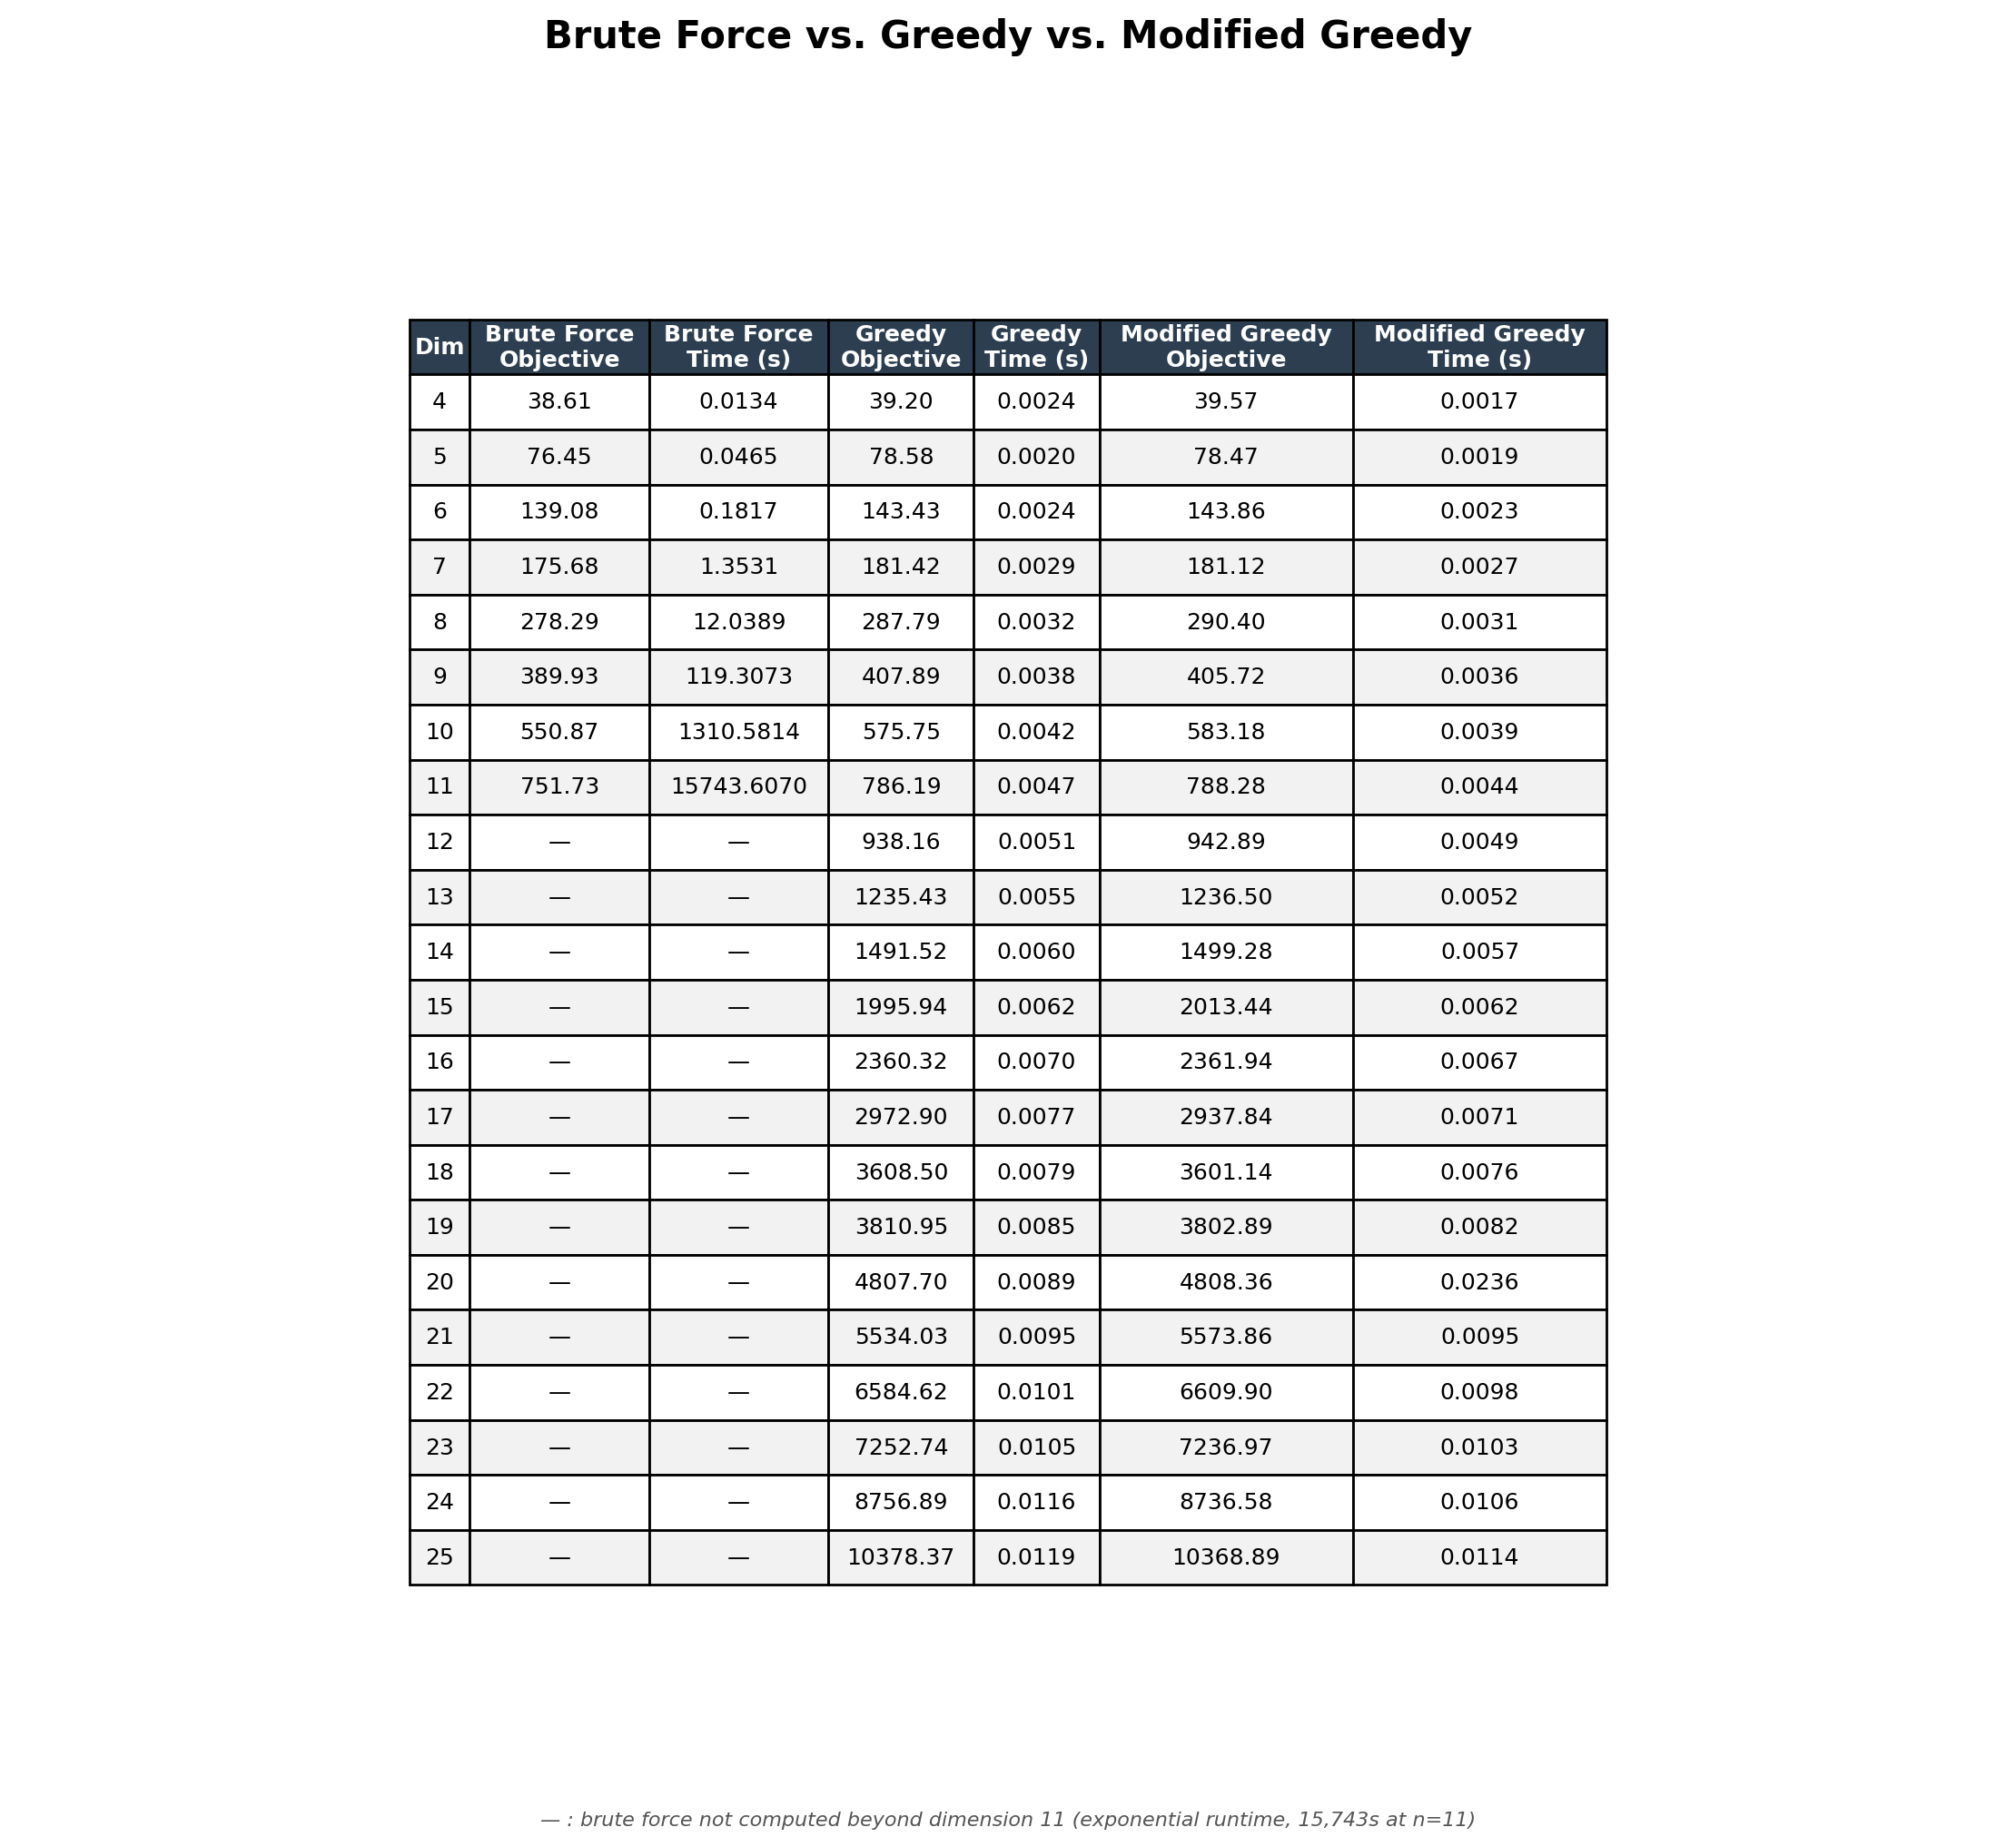
\includegraphics[width=0.95\textwidth]{table1_brute_greedy_modgreedy.png}
    \caption{Poredjenje brute force, greedy i modified greedy algoritama (prosek 10 instanci po dimenziji).}
    \label{fig:table1}
\end{figure}

Brute force algoritam daje optimalno rešenje, ali njegova vremenska
složenost raste eksponencijalno sa brojem taskova: vreme izvršavanja
skače sa $1310.58$ s za $n=10$ na $15743.61$ s (preko 4 sata i 20 minuta)
za $n=11$, odnosno raste više od $12$ puta pri uvećanju dimenzije za
samo jedan task. Zbog toga rezultati za $n > 11$ nisu dostupni (u tabeli
označeni sa "--") -- vreme izvršavanja bi bilo prakti\v{c}no neupotrebljivo.

Nasuprot tome, obe pohlepne heuristike izvršavaju se u zanemarljivom vremenu
($< 0.012$ s) nezavisno od dimenzije, ali po ceni kvaliteta rešenja. U opsegu
$n=4$--$11$, gde postoji egzaktno rešenje za poredjenje, \emph{greedy}
algoritam u proseku odstupa od optimuma za $3.48\%$, dok \emph{modified
greedy} odstupa za $3.85\%$. Zanimljivo je da modifikovana varijanta ne
daje konzistentno bolje rezultate od osnovnog pohlepnog algoritma -- za
pojedine dimenzije ($n=5,7,9,11$) daje čak nešto bolje rešenje, dok za
druge ($n=4,6,8,10$) daje lošije, što ukazuje da modifikacija menja
kriterijum izbora na način koji nije uniformno superioran, već zavisi od
strukture instance.

\subsection{S metaheuristike}

Tabela~\ref{fig:table2} uporedjuje brute force sa tri metaheuristike zasnovane
na lokalnoj pretrazi: \emph{local search}, \emph{Variable Neighborhood
Search} (VNS) i \emph{simulated annealing} (SA).

\begin{figure}[h!]
    \centering
    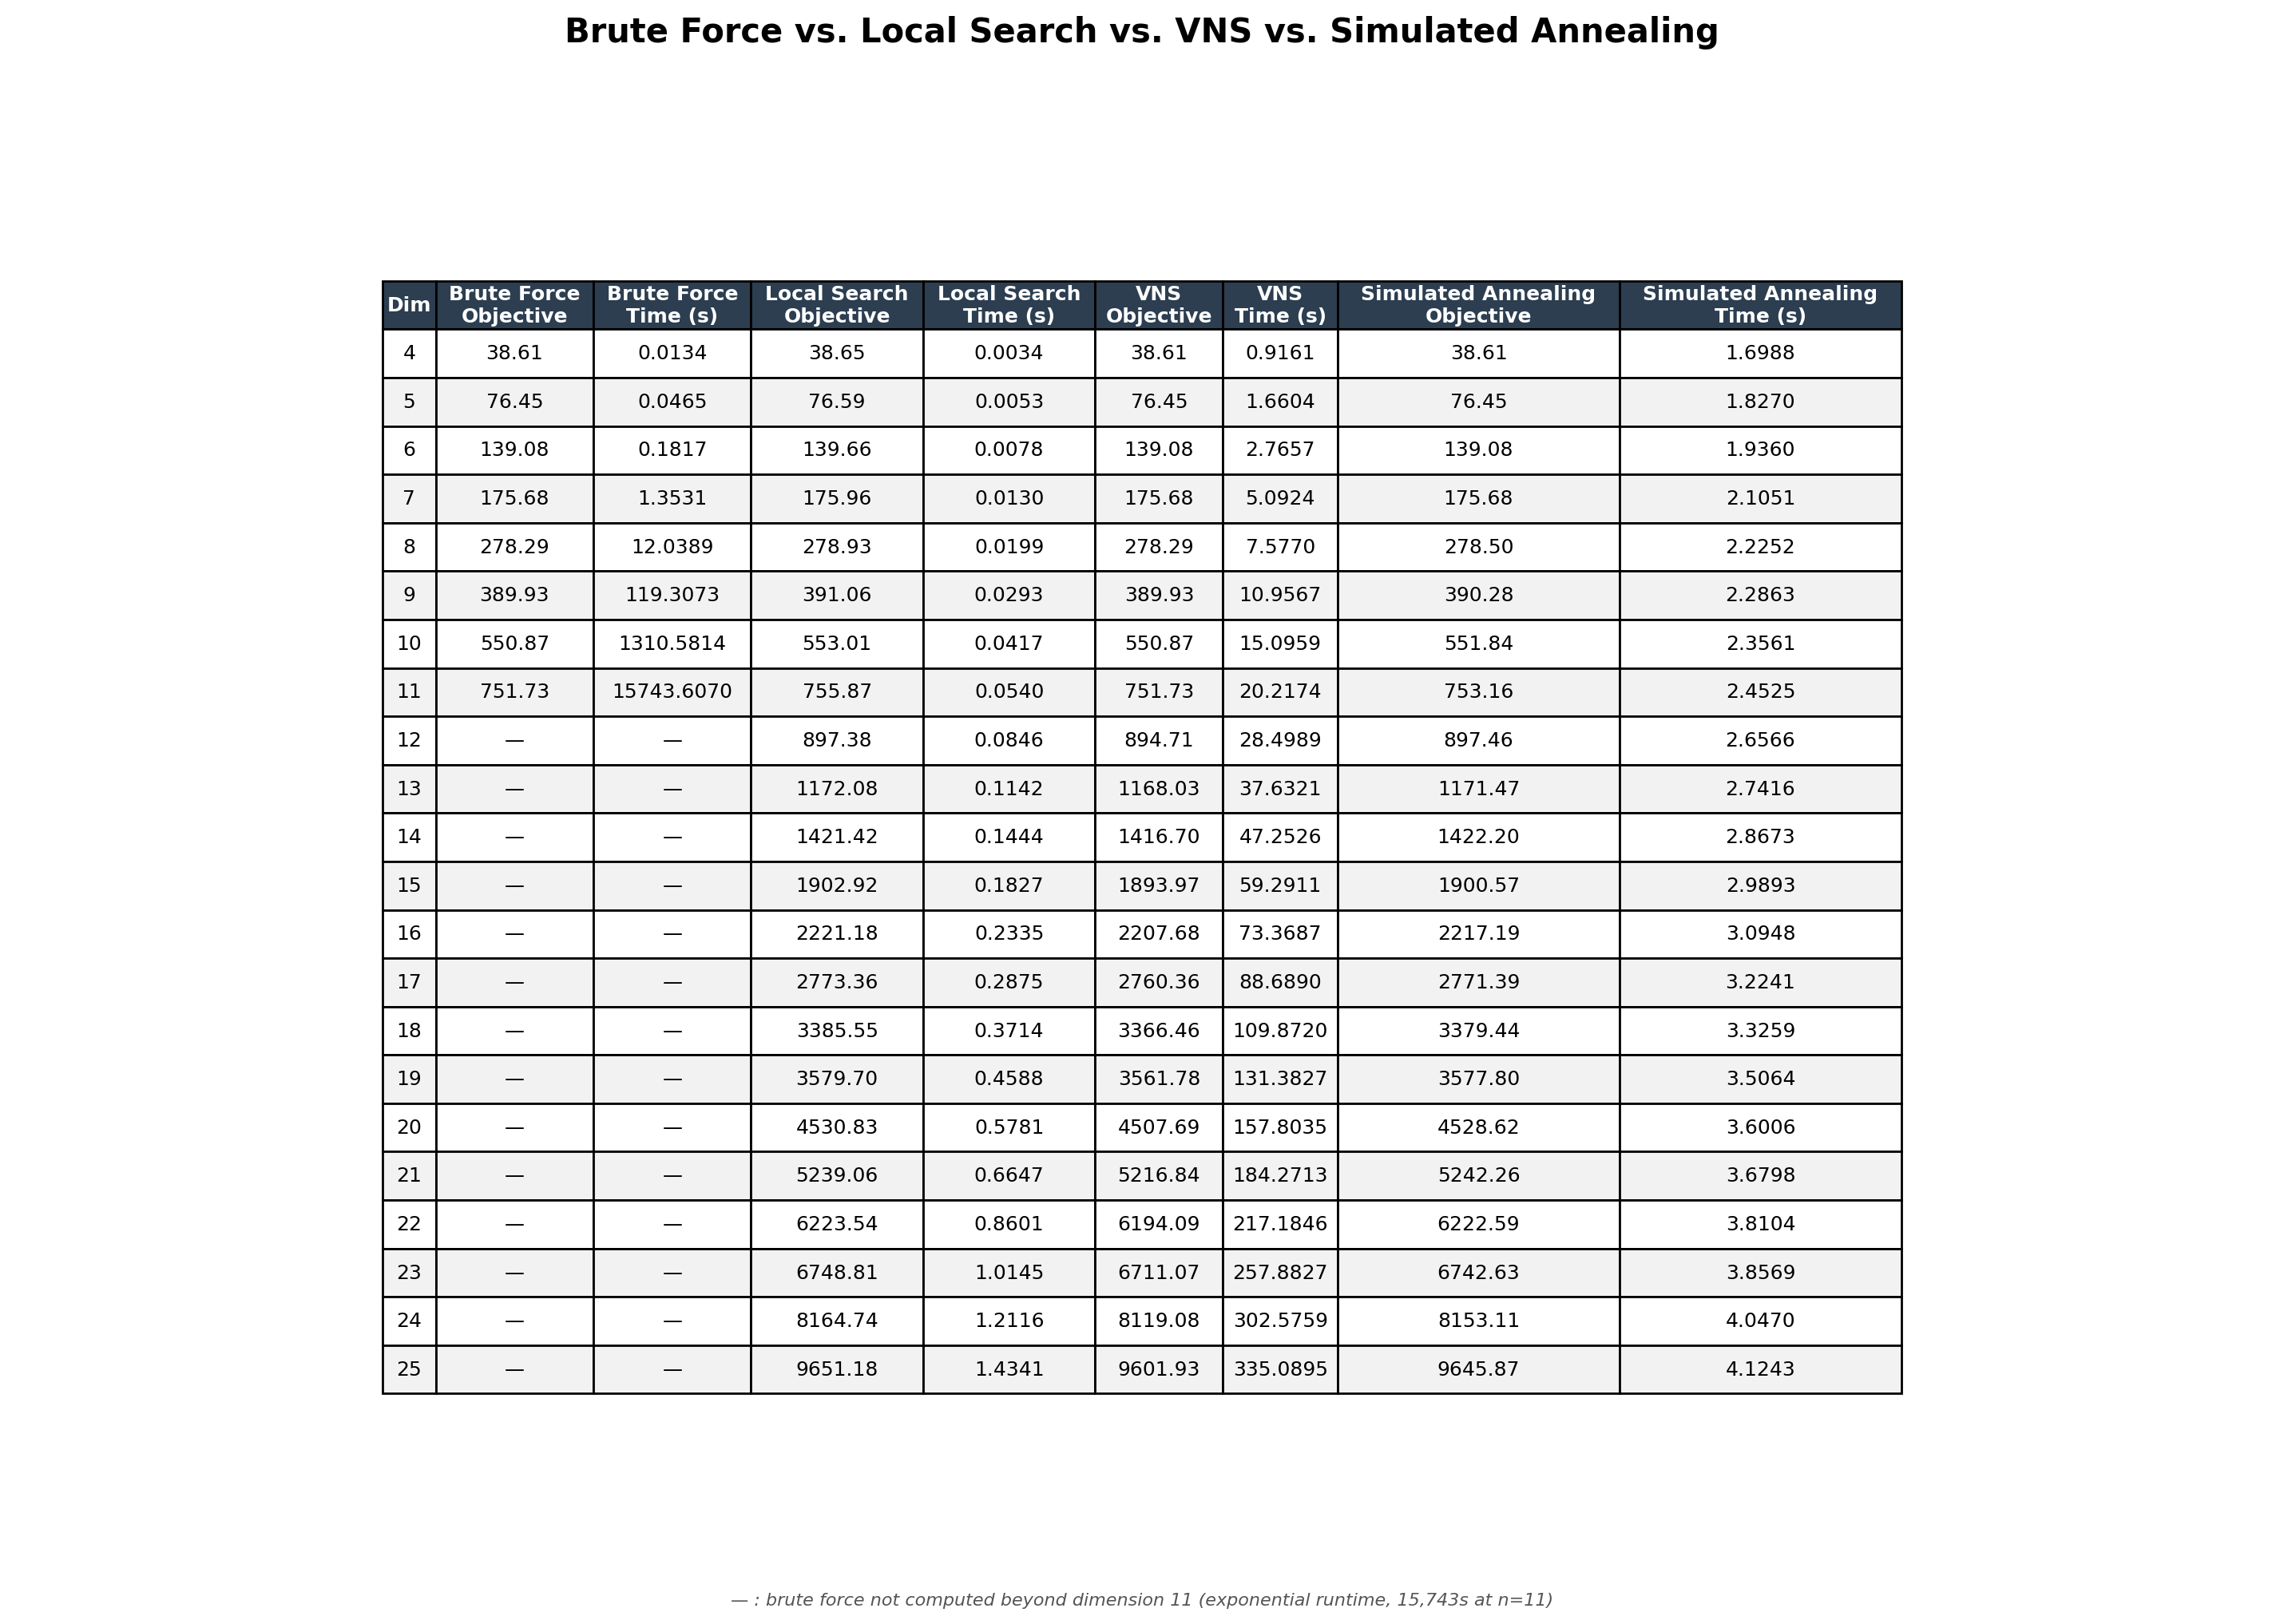
\includegraphics[width=0.95\textwidth]{table2_brute_ls_vns_sa.png}
    \caption{Poredjenje brute force, local search, VNS i simulated annealing algoritama (prosek 10 instanci po dimenziji).}
    \label{fig:table2}
\end{figure}

Sve tri metaheuristike znatno prevazilaze pohlepne heuristike po kvalitetu
rešenja. \textbf{VNS} u opsegu $n=4$--$11$ pronalazi optimalno rešenje u
svih 8 testiranih dimenzija, dok
\emph{local search} u proseku odstupa svega $0.29\%$, a \emph{simulated
annealing} $0.066\%$ od optimuma. Ovo je značajno poboljšanje u odnosu na
pohlepne konstrukcije, uz i dalje prihvatljivo vreme izvršavanja: za
najveću testiranu dimenziju ($n=25$) VNS-u je potrebno $335.09$ s, dok je
\emph{simulated annealing} znatno brži -- $4.12$ s -- uz rešenje vrlo
blisko VNS-ovom ($9645.87$ naspram $9601.93$). \emph{Local search} je pritom
najbrži od tri metode ($1.43$ s na $n=25$), što je očekivano jer izvršava
samo jedan prolaz do lokalnog optimuma bez mehanizma izlaska iz njega,
za razliku od VNS-a (koji sistematski menja susedstva) i SA-a (koji
prihvata i pogoršanja rešenja sa odredjenom verovatnoćom).

Ovi rezultati ukazuju na jasan \emph{trade-off} izmedju kvaliteta rešenja i
vremena izvršavanja: VNS daje najbolji kvalitet po ceni najdužeg vremena
izvršavanja (na $n=25$ oko $78\times$ sporiji od SA), dok je \emph{local
search} najbrži, ali sa najvećim odstupanjem od optimuma medju ove tri
metode.

\subsection{Populacioni algoritmi}

Tabela~\ref{fig:table3} uporedjuje brute force sa \emph{genetic algorithm}
(GA), \emph{memetic algorithm} (MA, GA obogaćen lokalnom pretragom) i VNS-om,
uzetim kao referentna vrednost iz prethodne tabele.

\begin{figure}[h!]
    \centering
    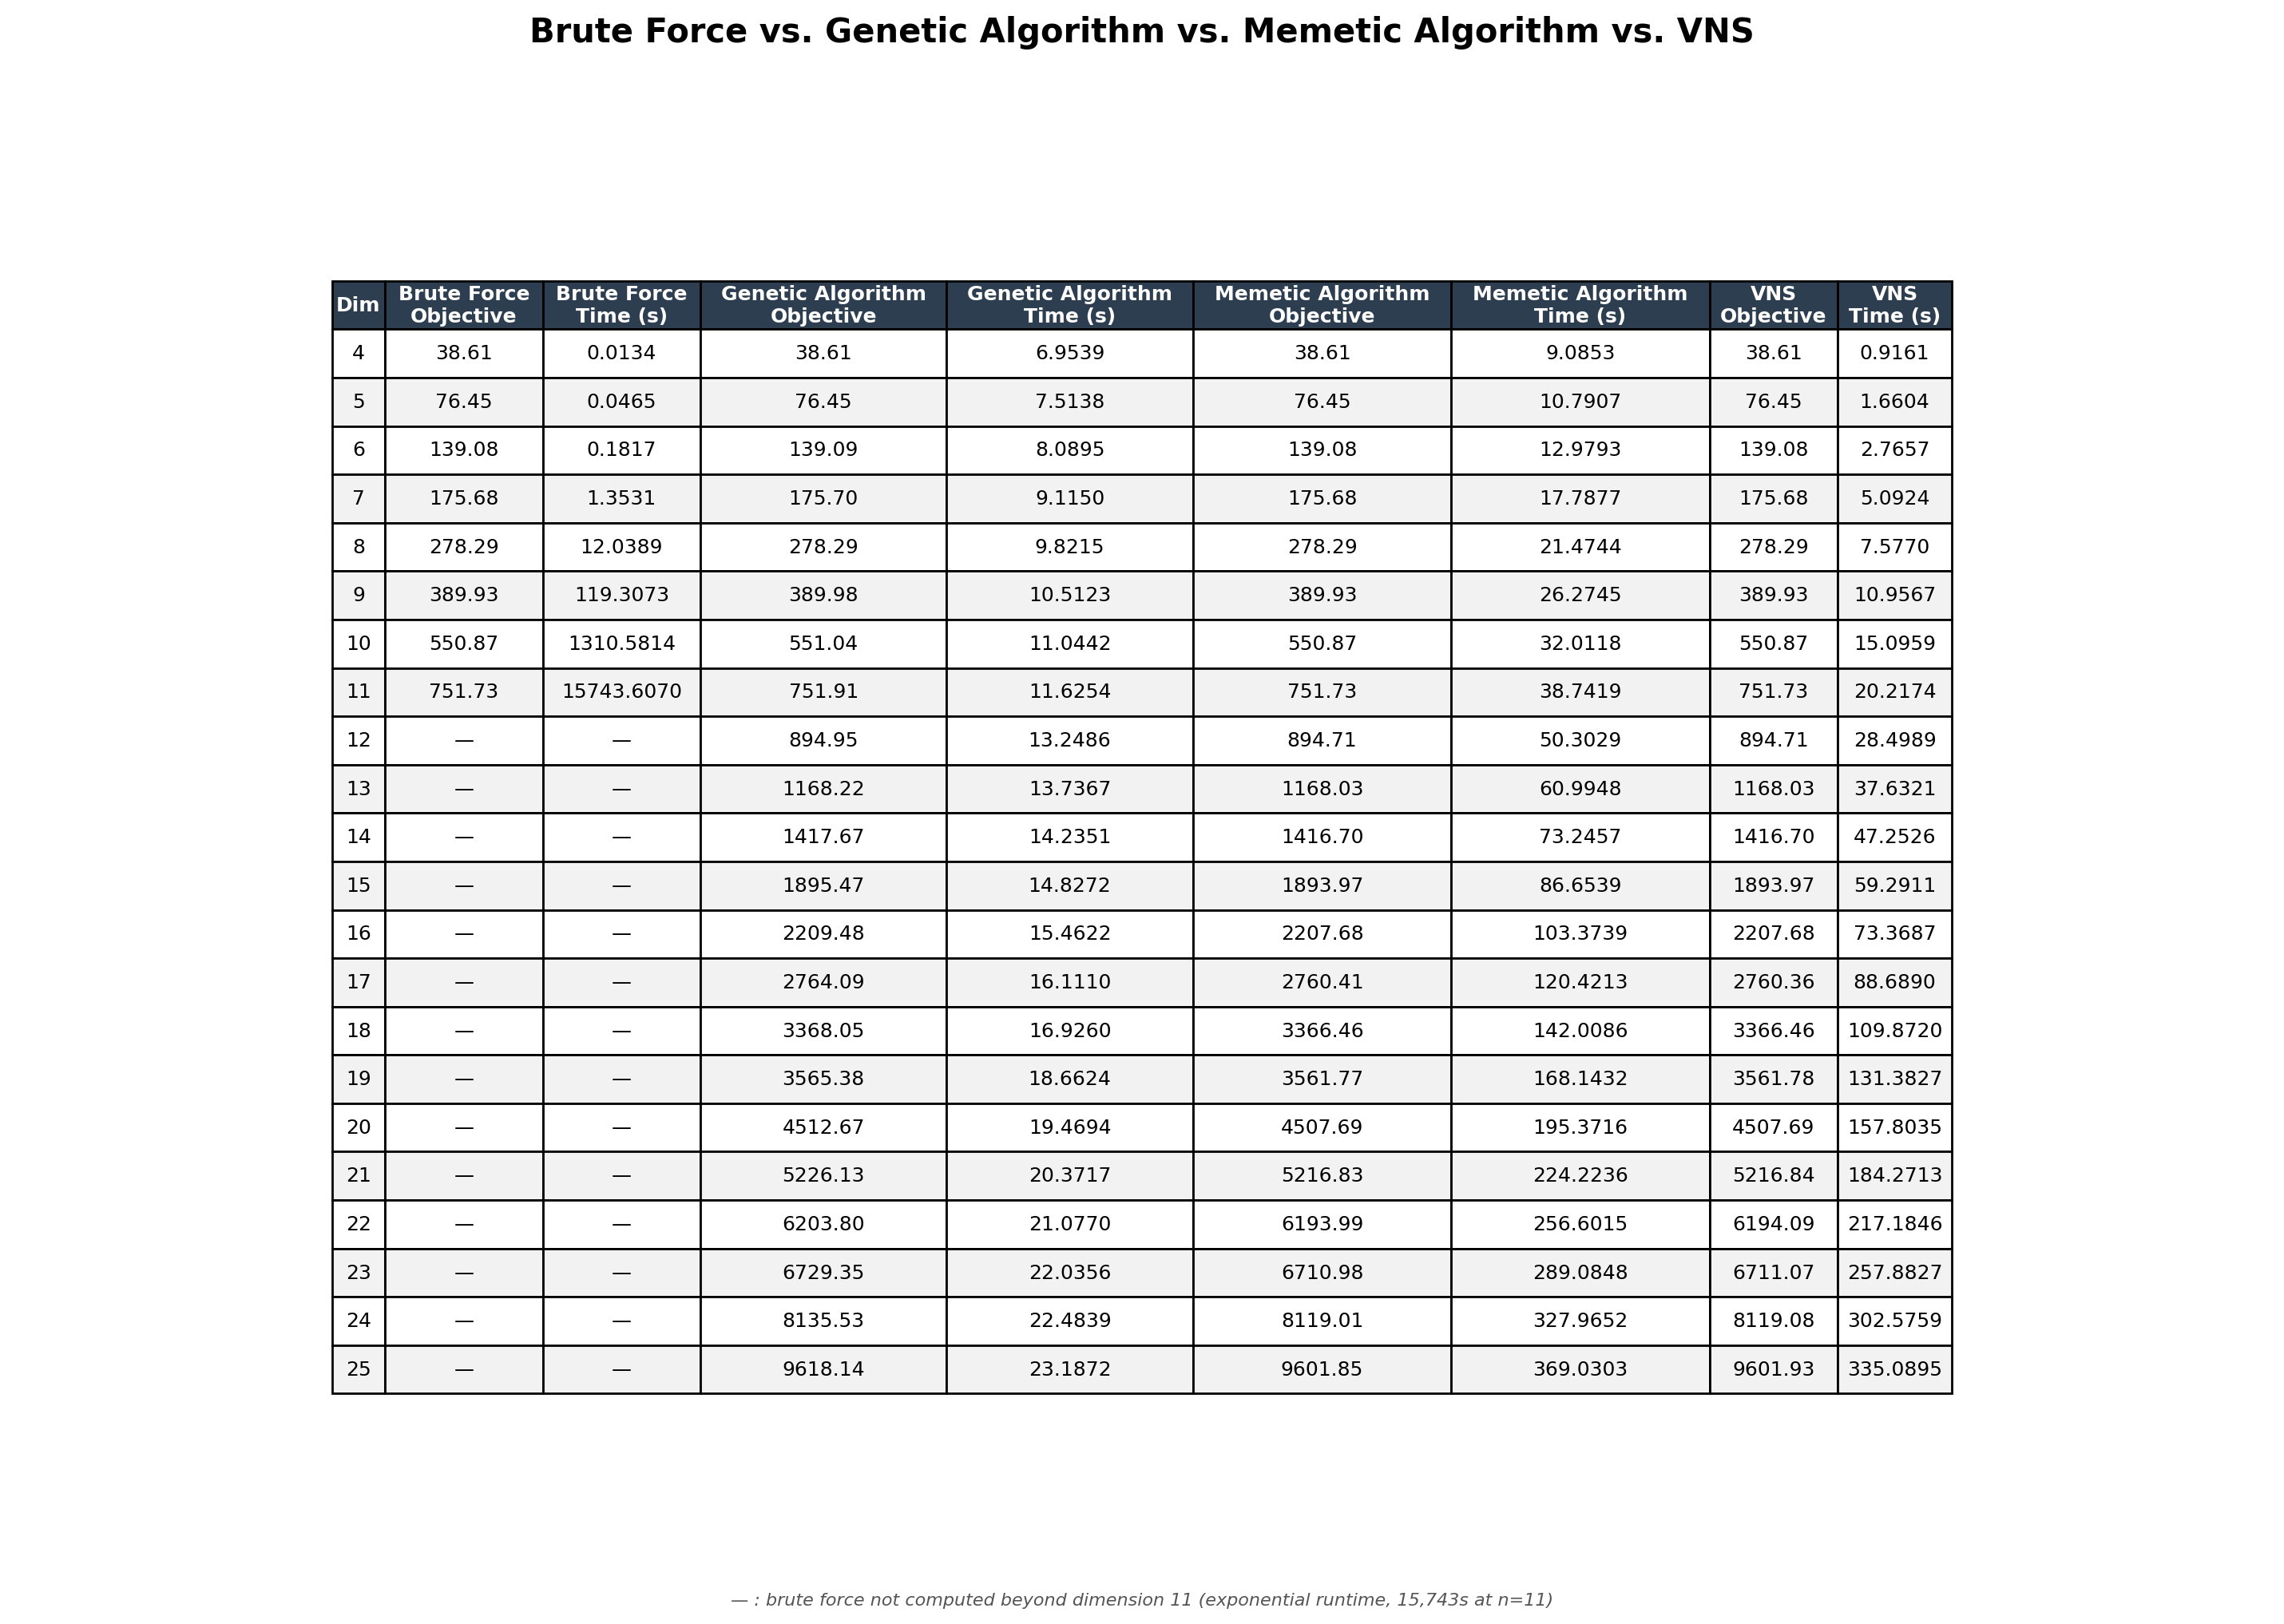
\includegraphics[width=0.95\textwidth]{table3_brute_ga_ma_vns.png}
    \caption{Poredjenje brute force, genetic algorithm, memetic algorithm i VNS algoritama (prosek 10 instanci po dimenziji).}
    \label{fig:table3}
\end{figure}

\emph{Memetic algorithm} pokazuje najbolje rezultate od sve tri metode:
u opsegu $n=4$--$11$ dostiže optimalno rešenje u svakoj testiranoj
dimenziji (prosečno odstupanje $0.00\%$), identično kao VNS, dok čist
\emph{genetic algorithm} u proseku odstupa svega $0.011\%$ od optimuma.
Iako je razlika u kvalitetu izmedju GA i MA mala, ona direktno potvrdjuje
očekivani efekat dodavanja lokalne pretrage u GA. Dosledno gura populaciju ka
optimalnim ili skoro optimalnim rešenjima, na račun dodatnog vremena
izvršavanja: na $n=25$, MA-u je potrebno $369.03$ s naspram $23.19$ s za
čist GA -- oko $16\times$ sporije, jer se lokalna pretraga poziva nad delom
populacije u svakoj generaciji.

Poredeći MA sa VNS-om, oba dostižu praktično identičan kvalitet rešenja
($9601.85$ naspram $9601.93$ na $n=25$), ali uz sličnu vremensku cenu
($369.03$ s naspram $335.09$ s). Čist \emph{genetic algorithm}, iako
neznatno lošijeg kvaliteta, ostaje znatno brži od obe metode ($23.19$ s na
$n=25$) i predstavlja razuman kompromis kada je vreme izvršavanja
kritičnije od poslednjeg procenta optimalnosti.

\section{Zaključak}

Rezultati potvrdjuju očekivanu hijerarhiju pristupa problemu minimizacije
težinskog vremena završetka:
\begin{itemize}
    \item \textbf{Brute force} garantuje optimalnost, ali je upotrebljiv
        samo za vrlo male instance ($n \leq 11$) zbog eksponencijalne
        složenosti.
    \item \textbf{Pohlepne heuristike} (greedy, modified greedy) su
        ekstremno brze, ali sa najvećim odstupanjem od optimuma
        ($\sim 3.5$--$3.9\%$).
    \item \textbf{Metaheuristike zasnovane na lokalnoj pretrazi} (local
        search, SA) postižu znatno bolji kvalitet
        ($< 0.3\%$ odstupanja), uz umeren do visok utrošak vremena. 
        VNS dostiže najbolji ili blizu najboljeg kvalitet rešenja.
    \item \textbf{Populacioni algoritmi} (GA, MA) dostižu najbolji ili
        blizu najboljeg kvalitet rešenja, gde MA (GA + lokalna pretraga)
        dosledno nadmašuje čist GA po kvalitetu, po ceni dodatnog vremena
        izvršavanja.
\end{itemize}

Za veće instance ($n > 11$), gde egzaktno poredjenje sa optimumom nije
moguće, VNS i memetic algorithm ostaju najkonzistentniji izbor kada je
kvalitet rešenja prioritet, dok su simulated annealing i genetic
algorithm bolji izbor kada je vreme izvršavanja ograničavajući faktor.

\end{document}